\section{Proposta: Segmentação Linear Automática de Atas de Reunião}
	\label{sec:proposta}






%%%%%%%%%%
% TextTiling e C99 criados para inglês e independente de domínio
%%%%%%%%%%
Os algoritmos \textit{TextTiling} e \textit{C99} foram propostos para o inglês, independentemente de domínio, ou seja, a proposta inicial dos autores é trabalhar em qualquer texto nessa língua.
%%%%%%%%%%
% Adapatar para Atas em português
%%%%%%%%%%
Assim, propõe-se aplicá-los ao contexto das atas de reunião em português do Brasil, ou seja, em uma língua diferente e dentro de um contexto específico. As subseções seguintes tratam da aplicação desses algoritmos para esse nicho mais específico. A Seção~\ref{sec:avaliacao} mostra a avaliação experimental e resultados obtidos.

%%%%%%%%%%
% Dificuldade: Coesão léxica não tão bem definida
%%%%%%%%%%
O vocabulário das reuniões, ainda que em tópicos diferentes, compartilham certo vocabulário pertencente ao ambiente onde se deram as reuniões. Isso é um fator que diminui a coesão léxica entre os segmentos.
%%%%%%%%%%
% Dificuldade: estilo da escrita
% - Paragrafo único
% - Cabeçalhos e rodapés
% - Pontuação --> ; encerrando sentenças
% - Insersão de espaços que não são quebra de sentença
% - Ruídos
%%%%%%%%%%
As atas de reunião costumam ter um estilo de escrita que deve ser levado em conta na aplicação dos algoritmos, como a identificação de finais de sentença na ausência de quebras de parágrafo, inserção de linhas que não separam assuntos, utilização de pontuação para transição de tópicos, e cabeçalhos e numerais ruidosos. 

Nas subseções a seguir serão apresentados o pré-processamento e a identificação de segmentos candidatos considerados para a segmentação de atas.





\subsection{Pré-processamento}
	\label{subsec:preprocessamento}

	O texto a ser segmentado frequentemente é extraído de documentos em formatos como \textit{pdf}, \textit{doc}, \textit{docx} ou \textit{odt}. Após a extração, uma ata tem em média 906 \textit{tokens}, incluindo elementos menos informativos, a fim selecionar as palavras mais significativas, o texto passa por processos de transformação os quais serão apresentados a seguir.
	

\begin{enumerate}


% Cabeçalhos e rodapés
\item Remoção de Cabeçalhos e rodapés: 
As atas frequentemente contém trechos que podem ser considerados pouco informativos e descartados durante o pré-processamento, como cabeçalhos e rodapés que se misturam aos tópicos tratados na reunião, podendo ser  inseridos no meio de um tópico e criando uma quebra que prejudica tanto o algoritmo de segmentação, quanto a leitura do texto pelo usuário.

% Identificação de sentenças
\item Identificação de finais sentenças: 
Cada final de sentença e identificado e marcado com uma \textit{string} especial, esse processo é melhor descrito na Subseção~\ref{subsec:indentificacaosentencas}.

% Limpeza
\item Limpeza: 
Todos os caracteres são convertidos em caixa baixa e elimina-se a acentuação, sinais de pontuação e todos os \textit{tokens} menores que três caracteres.

% Numerais
\item Remoção de numerais:
Nas atas, é comum o uso de numerais para marcação de páginas e linhas, da mesma forma, são pouco informativos e podem ser descartados.

% Stop Words
\item Remoção de \textit{Stop Words}: 
Remove-se as palavras consideradas menos informativas, para isso, utiliza-se uma lista contendo 438 palavras. 

% Stemming
\item \textit{Stemming}:
Extrai-se o radical de cada palavra, para isso, as letras são convertidas em caixa baixa e aplica-se o algoritmo \textit{Orengo}\footnote{\urlorengo} para remoção de sufixos.

\end{enumerate}
	
	

Após cada passo, os \textit{tokens} menos significativos são removidos e, ao final, são extraídas em média 441 palavras de cada ata, conforme mostrado na Tabela~\ref{tab:preprocessamento}.

%Testando Preprocessamento
%
%Loading docs         
%MÉDIAS --------------------> DOCS: 906.667
%
%Removing Headers     
%MÉDIAS --------------------> DOCS: 813.833
%
%Spliting sentences 
%Removing Punctuation 
%Removing Accents     
%Removing Shorters    
%MÉDIA  --------------------> DOCS: 535.333 | SENTENÇAS: 28.772
%
%Removing Numbers     
%MÉDIA  --------------------> DOCS: 526.500 | SENTENÇAS: 28.327
%
%Removing StopWords   
%MÉDIA  --------------------> DOCS: 441.000 | SENTENÇAS: 23.884
%
%Removing Stem  

\begin{table}[!h]
	\centering

	\begin{tabular}{|l|c|}
	
		\hline
		\textbf{Processo}      &  \textbf{Média de \textit{tokens}}\\		

		\hline

		Extração do texto                    & 906 \\ \hline
		Remoção de Cabeçalhos Rodapés        & 813 \\ \hline
		Identificação de finais de sentença  & 813 \\ \hline
		Limpeza                              & 535 \\ \hline
		Remoção de Numerais                  & 526 \\ \hline
		Remoção de \textit{Stop Words}       & 441 \\ \hline
		\textit{Stemming}                    & 441 \\ \hline
		
		
	\end{tabular}
	
	\caption{Quantidade média de \textit{tokens} extraídos após cada passo do pré-processamento.}
	\label{tab:preprocessamento}
\end{table}


A Figura~\ref{fig:exemplopreprocessamento} mostra a etapa de pré-processamento em uma sentença em português.
	


  \begin{figure*}
	\centering
	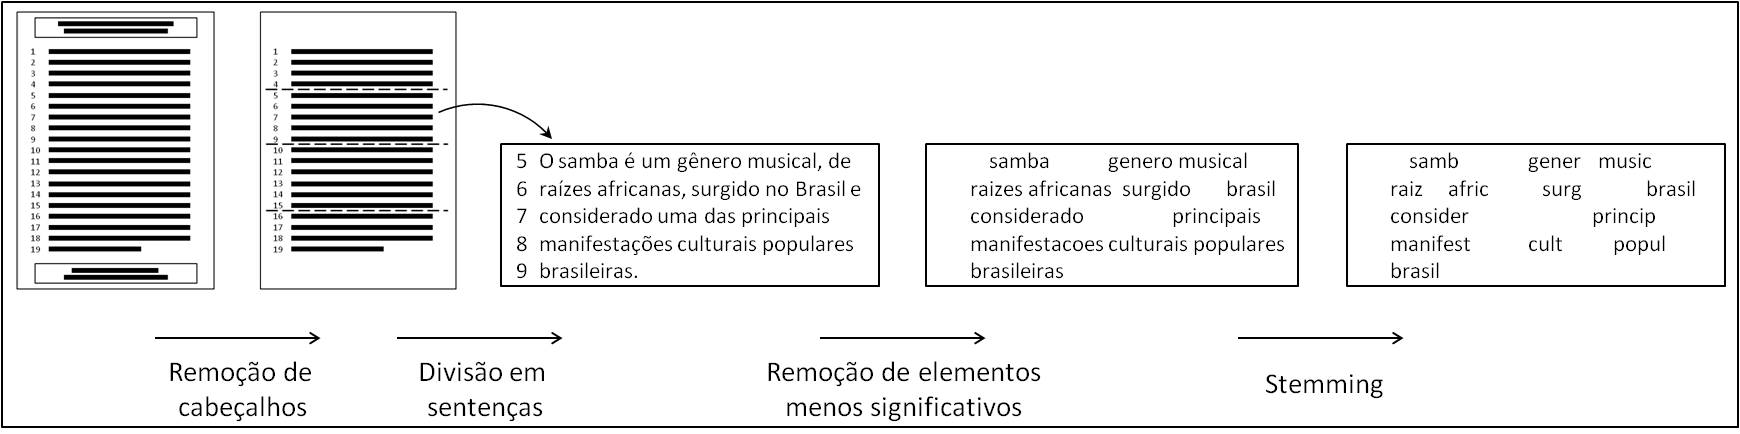
\includegraphics[width=1\textwidth]{pre-processamento.jpg}
	\caption{Exemplo de pré-processamento.}
	\label{fig:exemplopreprocessamento}
  \end{figure*}






\subsection{Identificação de candidatos}
	\label{subsec:indentificacaosentencas}
	
%%%%%%%%%%	
% Indicar unidade mínima de Segmento
%%%%%%%%%%
	
	
%	Como entrada para os 
%	Os algoritmos de segmentação devem ser
	É preciso fornecer aos algoritmos os candidatos iniciais a limites de segmento. Para isso, é necessário escolher qual será a unidade de informação mínima que constitui um segmento. Baseando-se no estilo de escrita e considerando as pontuações de um texto, é possível, em alguns casos, indicar quebras de parágrafo, finais de sentenças ou mesmo palavras como elementos que encerram um segmento. 

	Ocorre que em atas de reunião é uma prática comum redigi-las de forma que o conteúdo discutido fica em parágrafo único, além disso, as quebras de parágrafo são usados para formatação de outros elementos como espaço para assinaturas. 
%
	Também não é conveniente indicar todo ponto entre \textit{token} como candidato pois obrigaria a ajustar posteriormente os segmentos de maneira a não quebrar uma ideia ou frase. 
%	
	Assim, neste trabalho, os finais de sentença são considerados unidades de informação e portanto, passíveis a limite entre segmentos. 
	
	Devido ao estilo de pontuação desses documentos, como encerrar sentenças usando um \textit{";"} e inserção de linhas extras, foram usadas as regras apresentadas no Algoritmo 1 para identificar os finais de sentenças.  


\begin{algorithm}
	\SetKwInOut{Input}{Entrada}
	\SetKwInOut{Output}{Saída}
	\SetKwBlock{Inicio}{início}{fim}
	\SetKwFor{ParaTodo}{para todo}{}{fim para todo}
	\SetKwIF{Se}{SenaoSe}{Senao}{}{}{senao se}{senao}{fim se}
	\SetKwFor{Para}{}{}{}
%	\SetKwAlgorithm{Algorithm}{Algoritmo}{}

	
	\Input{Texto}
	\Output{Texto com identificações de finais de sentença}
	
	\ParaTodo {token, marcá-lo como final de sentença se:} {	

	Terminar com um \texttt{!}\\
	Terminar com um \texttt{.} e não for uma abreviação\\
	Terminar em \texttt{.?;} e:
		\Para{}{
			For seguido de uma quebra de parágrafo ou tabulação\\
			O próximo \textit{token} iniciar com  \texttt{(\{["'}\\
			O próximo \textit{token} iniciar com letra maiúscula\\
			O penúltimo caracter  for \texttt{)\}]"'}\\
		}
	}
	
	\caption{Identificação de finais de sentença}
	\label{alg:identificacaofinaisdesent}
\end{algorithm}





%conforme mostrado no Algoritmo~\ref{alg:identificacaofinaisdesent}.
%	
% 2) Eliminação de ruídos
%\item \textit{Remoção de ruídos}:
%%%%%%%%%%
% Remoção de ruídos
%%%%%%%%%%
%Nesse trabalho, esses elementos são removidos, uma vez que, o descarte não causa perca de informação e pode facilitar a identificação dos segmentos, pois melhora a coesão do texto. Outro benefício é manter o texto livre de trechos que fogem do assunto circundante.
%%%
% TODO: Como são removidos?
% por meio de heurísticas simples
%%%

%Elimina-se também nesse passo a acentuação, sinais de pontuação, restando apenas palavras.  






%Como forma de padronização, as instituições acrescentam ao documento

%		passos menores
%		1 - heurística simples para remover cabeçalho e rodapé.
%		2 - remoção de numerais
%		3 - remoção de acentos, transformações de caixa, remoção de pontuação.
		
	% Esses passos são realizados internamente em cada algorímo, para que a saida seja legível ao usuário final.





%A qualidade do algoritmo é sempre dependente da escrita correta! Ausência de emoticons, códigos de computador e gírias.





%Nas subseções a seguir serão expostas as alterações para aumentar a eficiência dos algoritmos e encontrar o melhor modelo para a tarefa de segmentar o texto das atas em tópicos.



%Tais aspectos não se aplicam ao contexto das atas, onde o estilo de escrita em forma de narrativa, prefere poupar o leitor de diálogos secundários durante transições de tópicos. 







	
	
%Elimina-se textos considerados de pouca relevância como a numeração de páginas e linhas, cabeçalhos e rodapés, também elemina-se acentuação, sinais de pontuação, restando apenas palavras.  


	
	
%%
%% 1) Identificação de sentenças
%Primeiro cada final de sentença e identificado e marcado com uma \textit{string} especial, esse processo é melhor descrito na Subseção~\ref{subsec:indentificacaosentencas}.
%%
%%conforme mostrado no Algoritmo~\ref{alg:identificacaofinaisdesent}.
%
%%	
%% 2) Eliminação de ruídos
%Depois, elimina-se textos considerados de pouca relevância como a numeração de páginas e linhas, cabeçalhos e rodapés, também elemina-se acentuação, sinais de pontuação, restando apenas palavras.  
%
%%	
%% 3) Stop Words
%Em seguida, remove-se as palavras consideradas menos informativas, as quais são chamadas de \textit{stop words}, para isso, utiliza-se uma lista contendo 438 palavras. 
%
%%
%% 4) Stemming
%Por fim, extrai-se o radical de cada palavra, para isso, as letras são convertidas em caixa baixa e aplica-se o algoritmo \textit{Orengo}\footnote{\urlorengo} para remoção de sufixos.
%
%
%Tem-se então, uma lista com os elementos considerados mais significativos do texto. A Figura~\ref{fig:exemplopreprocessamento} mostra a etapa de pré-processamento em uma sentença em português.
%	





